\documentclass{article}

\usepackage[utf8]{inputenc} 
\usepackage{outlines}
\usepackage{amsmath}
\usepackage{cleveref}
\usepackage{graphicx}
\usepackage{xr}
\usepackage{siunitx}

\usepackage[margin=1in]{geometry}
\parskip 1.5ex % paragraph spacing

\graphicspath{./docs/Figures/}

\title{Variation in thermal sensitivity drives patterns of species richness across thermal gradients}
\author{Tom Clegg, Samraat Pawar}
\date{January 2021}

\begin{document}

\maketitle

\section{Introduction}

The effect of temperature on species richness has long been a topic of interest in ecology (REF). Starting with the pioneering work of Alexander von Humboldt, who in the 19th century identified temperature as a major environmental driver of plant richness along elevational gradients in the Andes (REF), clear relationships between richness and temperature have been identified across many different taxa and environments ranging from aquatic microbes (REF) to terrestrial tree communities (REF). 

Unsurprisingly the existence of these patterns has resulted in various attempts to explain the role of temperature in driving species richness (REF), evoking a range of mechanisms focused on the effects of temperature on both ecological (e.g. the effects of temperature on metabolism and population demography; (REF)) and evolutionary (e.g. the effects of temperature on mutation rate and generation time; (REF)) processes. Most notably these were synthesised into a single framework in a series of papers (hereafter referred to as the "metabolic theory of biodiversity" (MTB) (REF)) as an extension of the metabolic theory of ecology (REF), which aimed to explain the effects of temperature on biodiversity through the link between individual metabolic rate and the various ecological and evolutionary processes that control species richness (REF). One of the central predictions made by MTB is that species richness should follow an simple, monotonic Arrhenius-type response with a single temperature sensitivity equal to the assumed universal value for metabolism (REF). This means that the natural log of species richness should follow a linear relationship when plotted against $\frac{1}{kT}$, where $k$ is the boltzmann constant (\SI{8.617e-5}Ev) and $T$ is temperature in Kelvin, with a slope of $\sim 0.65$ (REF).

Despite the attractiveness of it's simplicity and the apparent support of early tests with empirical data, MTB has received considerable criticism since its initial publication. Most of this has been focused on further tests of its central prediction, which revealed limited support for the single global temperature dependence of richness (REF). In separate analyses across both latitudinal (REF) and elevational (REF) gradients species richness was observed to demonstrate thermal responses that both varied in shape, deviating from the predicted monotonic Arrhenius form, and in magnitude (i.e. deviating from $E = 0.65$). In response to this discrepancy Stegan et al. proposed and extension to MTB, using a more general, trait-based eco-evolutionary framework. This framework provided a more "integrated" approach to MTB, explicitly including the temperature dependence of various ecological and evolutionary processes such as interactions between species, mortality and mutation rates, generating species richness temperature relationships that displayed similar variation to those seen in empirical data. One aspect that was not explored in this model however was variation in thermal sensitivity, with the authors assuming (like most work as part of the metabolic theory of ecology) that thermal sensitivity of different processes and populations took the single "universal" value of $E=0.65$ across the different ecological processes and taxa, an assumption based on the average thermal sensitivity of the respiratory complex which in turn, determines the thermal response of basal metabolic rate (REF).

Despite its success in predicting broad scale macroecological patterns (REF), this assumption of a single temperature dependence ignores the widespread variation in thermal sensitivity that has been observed across the tree of life. This variation has been documented in number of studies looking at thermal sensitivity both across different taxa (REF) and ecological processes (REF) and has been highlighted as a potentially important factor in determining the response of ecological systems to temperature. For example "thermal mismatches", the differences in the thermal responses between different species or ecological processes, have been shown to be potentially important in a number of contexts such as consumer-resource (REF) and parasite-host systems (REF). Furthermore, the non-linear nature of temperature responses mean that considering only the average thermal response (and thus ignoring all higher-order moments) is unlikely to be a good approximation if significant variance in thermal sensitivity exists (see REF for a similar discussion in regards to variance in temperature and its effect on thermal performance curves). It follows then that variation in thermal responses will be important in driving patterns of species richness which are driven, at least in part, by processes sensitive to variation (e.g. interspecies interactions) and non-linear thermal responses. 

In this paper we investigate the effects of of variation in thermal sensitivity and its role in driving patterns of species richness over temperature gradients. Using a general model of ecosystem dynamics we first derive analytical results, explicitly linking the variation in thermal sensitivity to the numbers of species within ecosystems and thus patterns in species richness. Then, using a newly assembled dataset of bacterial species growth curves we obtain estimates for actual variation in thermal sensitivity and show that over relevant parameter space, variation is indeed important in driving patterns of species richness over temperature. We then we test these predictions using numerical simulations of assembly in complex species-rich communities, showing these analytical predictions are robust when relaxing assumptions about ecosystem dynamics.  

\section{Methods}
\subsection{Theory}
 We start by first deriving an analytical expression for species richness in terms of temperature. Broadly our approach here is to first to derive an expression for the maximum number of species a single community with a given distribution of demographic traits (i.e. growth rates and interaction strengths) can support without extinctions occurring. This property is also known as feasibility and is itself often discussed in relation ecological stability analysis (REF). We then establish how temperature (via its effects on population demographic rates and interactions) affects the feasibility of systems and how this relationship is modified by variation in thermal sensitivity. Combined, these two insights allow us to link the effects of variation in thermal sensitivity on species richness through its effects on the feasibility of ecosystems. 

\subsubsection{Model}
In order to explore the effects of temperature on species richness we use the generalised Lottka-Volterra model (GLV) (REF). This framework is commonly used to explore ecosystem dynamic properties and is regularly applied to study complex, multi-species communities (REF). The GLV describes the dynamics of an $N$ species community where the growth of species $i$ is given by:

\begin{equation} \label{EQ:GLV}
  \frac{1}{x_i} \frac{dx_i}{dt} = r_i(T) - a_{ii}(T) x_i - \sum^N_{i \neq j} a_{ij}(T) x_j, 
\end{equation}

where $x_i$ is the biomass of the $i$th species, $r_i(T)$ is it's intrinsic growth rate, determining the rate at which new biomass is produced ($\text{mass} \cdot \text{time}^{-1} \cdot \text{mass}^{-1} $) and $a_{ij}(T)$ describes the effect of interactions with species $j$ on $i$ (with the $a_{ii(T)}$ term representing intraspecific interactions; $\text{mass}^{-1} \cdot \text{time}^{-1}$). Note that both parameters are expressed as functions of temperature, the form of which will be discussed later.  

As we want to determine the number of species this community can support we first derive an expression for the equilibrium biomass. Though it is not possible to derive an exact analytical solution for the GLV as described in \cref{EQ:GLV}, we use a mean-field approximation, developed by (REF) to get estimate of equilibrium biomass. In brief, this approximation works by considering the effect of interactions not in terms of their individual pairwise components (i.e. the last term of \cref{EQ:GLV}) but in terms of the average effect of interactions across the community, assuming the system we consider is large and that no individual pairwise interaction dominates the dynamics (see \cref{SI_Sec:Meanfield} for more detail). This gives the expression: 

\begin{equation}\label{EQ:MF_equi}
  x^*_i \approx K_i(T) -  \bar{K}(T)  \frac{ (N-1)\bar{a}(T)}{1 + (N-1)\bar{a}(T)}, 
\end{equation}

where $K_i = \frac{r_i(T)}{a_{ii}(T)}$ is the carrying capacity, the biomass a population would reach if grown in isolation (obtained by solving \cref{EQ:GLV} with no interactions) and $\bar{a}(T)$ is the average pairwise interaction strength. Overall \cref{EQ:MF_equi} provides an intuitive expression for the equilibrium biomasses; a population will reach the biomass that it would in isolation (first term of the RHS, $K_i(T)$) minus the effects of any interspecific interactions (second term on RHS). The strength of these interspecific effects is determined by the average carrying capacity of heterospecifics ($\bar{K}(T)$) and a saturating function of total interaction strength experienced by the focal species, $(N-1)\bar{a}(T)$. If interactions are overall competitive (i.e. $ \bar{a}(T) > 0$) then we see a reduction in equilibrium biomass relative to the individual carrying capacities whereas if they are facilitatory ($ \bar{a}(T) < 0$) we see an increase.  

\subsubsection{Feasibility and Species Richness} \label{SEC:Feas_SP_rich}
Next we use \Cref{EQ:MF_equi} to derive an expression for community feasibility (the capacity of a system to maintain positive biomasses for the species within (REF)) in terms of the population demographic parameters (i.e. the $r(T)$'s and $a(T)$'s) which will then be used to determine the upper bound on species richness $N$. We start with the definition that a system is feasible if all species have non-zero equilibrium biomass (i.e. $x_i^* > 0 $; REF), giving the condition:

\begin{align} \label{EQ:Feas_sp}
  \kappa_i(T) > \frac{(N-1)\bar{a}(T)}{1 + (N-1)\bar{a}(T)} \quad \text{for all} \quad i = 1 \ldots N,
\end{align}

where $\kappa_i = \frac{K_i(T)}{\bar{K}(T)}$ is the mean-normalised carrying capacity. \Cref{EQ:Feas_sp} shows how a system is feasible as long as the the effects of interspecific interactions on the each population (RHS) do not outweigh the growth rates and intraspecific interactions (LHS). We can see that in the case of facilitatory interaction ($\bar{a}(T) < 0$) the inequality will always hold and the system will be feasible. Only when interactions are on average competitive (i.e $\bar{a}(T) > 0$) will they be enough to make the system unfeasible. 

Using \cref{EQ:Feas_sp} we formulate an expression for the probability of feasibility $P_{feas}$, the probability that a community is feasible given the distribution of species trait values ($\kappa$s and $a$s) and number of species ($N$) in the system. To do so we take \cref{EQ:Feas_sp} and consider $\kappa$ and $a$ as random variables, each describing the distribution of the respective traits across the populations in the community (represented in notation by the loss of subscript). This lets us consider $\kappa$'s cumulative density function (CDF) which gives the probability that $\kappa$ is less than or equal to some value, $F_{\kappa}(x,T) = P(\kappa \leq x)$. As the condition for feasibility states that $\kappa$ must be greater than the effect of interactions we can apply the CDF to \cref{EQ:Feas_sp} and write $P_{feas}$ as:

\begin{equation} \label{EQ:P_feas}
    P_{feas}(T) = P \left( \kappa(T) > \frac{(N-1)\bar{a}(T)}{1 + (N-1)\bar{a}(T)}  \right)^N = 
    \left[1 - F_{\kappa}\left(\frac{(N-1)\bar{a}(T)}{1 + (N-1)\bar{a}(T)},T \right)\right]^N,
\end{equation}

giving the probability of feasibility of an ecosystem as a function of the species traits (\cref{Fig:P_feas}). Note the expression is raised to the $N$th power as the term in the brackets must hold for all $N$ populations in a community for it to be feasible.

\Cref{EQ:P_feas} makes explicit the effect of species richness $N$ on the probability of feasibility in a community, showing how $P_{feas}$ will decline with increasing $N$ through two mechanisms. Firstly it alters the strength of interactions experienced by individual populations via the $(N-1) \bar{a}(T)$ term. A higher species richness means that the strength of interactions will be greater and if interactions are on average competitive ($\bar{a}(T) < 0$) this will reduce the probability of feasibility. Secondly, the probability of feasibility will fall as the number of species increases as it becomes less likely that all $N$ species meet the criteria in \cref{EQ:Feas_sp} as represented by the $N\text{th}$ power term in \cref{EQ:P_feas}. 

Importantly this decline in $P_{feas}$ with increasing richness places an upper bound on species richness given a certain distribution of $\kappa$ and $a$ values within a community. If a system is too large then we expect that it will have a low probability of feasibility and thus be likely to experience population extinctions until the probability of feasibility becomes larger and extinctions become unlikely. Though ideally we would use \cref{EQ:P_feas} to determine this bound explicitly by solving for $N$ this is not possible for most distributions of $\kappa$ due to the complexity of their CDFs. We therefore use a numerical approach to determine the exact value of this upper bound on $N$ (see SECTION XX). It is important to note that this does not preclude us gaining insight into the effects of variation in thermal sensitivity which are discussed in more detail in \cref{SEC:Temperature}. 

\subsection{Temperature} \label{SEC:Temperature}
Having defined the relationship between species richness and the distribution of demographic rates and interactions across the community we now turn to the effect of temperature. Broadly our approach here is to consider how the distributions of the relevant species traits across populations change with temperature and thus $P_{feas}$ and the upper bound on $N$. Crucially we derive expressions for these temperature dependent distributions in terms of the distributions of thermal sensitivity parameters, allowing us to assess the effect of variation in thermal sensitivity between both populations and different traits on the temperature-species richness relationship. As discussed above this approach is motivated by the large body of empirical and theoretical work demonstrating the existence and consequences of the temperature dependence of these population processes and the variation that exists in these responses. Overall this temperature dependence can be explained by the dependence of these processes on metabolic rate (REF) which determines the capacity of individuals to growth and interaction with one another and is in turn affected by temperature through its effects on biochemical kinetics (REF).

Following the metabolic theory of ecology (REF) we use the modified Boltzmann-Arrhenius equation to represent the temperature dependence of $\kappa$ and $a$, which describes the exponential-like increase of some process with temperature (REF). Though empirically measured temperature response curves tend to have a uni-modal shape, we use the Boltzmann-Arrhenius due to its analytic tractability and its ability to capture the rising portion (before the temperature peak) of these curves (REF). We focus on this part of the curve as it is expected that the range of temperatures individuals actually experience (their operational temperature range) tends to below this thermal peak, making the exponential portion more relevant for the dynamics of real ecosystems (REF). This form of the Boltzmann-Arrhenius uses two parameters to describe the thermal response of a some process $B(T)$, the normalisation constant $B_0$ which is the value at a reference temperature and thermal sensitivity $E$ which determines the magnitude of the response of $B(T)$ to changes in temperature:

\begin{equation} \label{EQ:Boltzmann}
    B(T) = B_0 e^{-\frac{E}{k} \left(\frac{1}{kT} - \frac{1}{k T_{ref} }\right)},
\end{equation}

where $k$ is the Boltzmann constant and $T$ and $T_{ref}$ are the temperature and reference temperature (in kelvin) respectively. Applying \cref{EQ:Boltzmann} allows us to characterise the distributions of parameters across species populations at different temperatures in terms of the distributions of the underlying thermal sensitivity parameters ($B_0$s and $E$s). Assuming that the parameter values follow a log-normal distribution (a natural assumption given the exponential form of \cref{EQ:Boltzmann}), we obtain an expression for the temperature dependent distribution of $B(T)$ (see \cref{SI_Sec:TPC_dist}):

\begin{align} \label{EQ:Boltz_dist}
    \log(B(T)) \sim \mathcal{N}\left(\mu_{B}(T) , \sigma_{B}^2(T) \right) 
    \quad \text{where} \quad
    \begin{array}{cc}
        \mu_B(T) &= \mu_{B_0} - \mu_{E} \left(\frac{1}{kT} - \frac{1}{k T_{ref} }\right)  \\
        \sigma_{B}(T)^2 &= \sigma_{B_0}^2 + \sigma_{E}^2 \left(\frac{1}{kT} - \frac{1}{k T_{ref} }\right)^2
    \end{array}
\end{align}

where $\log(B_0)$ and $E$ are both normally distributed, with $\mu$ and $\sigma^2$ representing their mean and variance respectively. \Cref{EQ:Boltz_dist} makes explicit the effect of the distribution of thermal sensitivity parameters on the distribution of $B(T)$ showing that the sign and magnitude of the temperature response is controlled by a combination of the the average thermal sensitivity, $\mu_E$, as a linear function of temperature and the variance term $\sigma_E$, which introduces an additional quadratic term, creating additional curvature in the thermal response. The distribution of normalisation constants $B_0$s is present simply as an constant term in the expressions for both mean and variance. It is important to note here that as $B(T)$ is log-normally distributed it's moments are defined in terms of both the mean and variance in \cref{EQ:Boltz_dist} and thus both temperature dependent factors (the linear and quadratic parts) will contribute to the shape of the distribution. Applying \cref{EQ:Boltz_dist} to the distributions of $\kappa$ and $\bar{a}$ as defined in the \cref{SEC:Feas_SP_rich} we obtain the expressions:

\begin{align} \label{EQ:Trait_distributions}
        \log(\kappa(T)) &\sim \mathcal{N}\left( -\frac{\sigma_{K}^2(T)}{2} , \sigma_{K}^2(T) \right) \quad \text{and} \\ \nonumber \\
        \bar{a}(T) &= \exp \left(\mu_a(T) + \frac{\sigma_a^2(T))}{2} \right),
\end{align}

which show how the temperature responses of $\kappa$ and $\bar{a}$ are determined by the distributions of thermal response parameters. Importantly we see that the variance terms are present in both expressions meaning that the curvature introduced by the quadratic temperature term in \cref{EQ:Boltz_dist} will be present. Overall \cref{EQ:Boltz_dist,EQ:Trait_distributions} provide heuristic insight into the effects of the distribution of thermal sensitivities in the species richness curve. The average thermal sensitivity of $a$ will control the direction and magnitude of the temperature response whilst the average for $K$ will have no effect (as the average does not affect the distribution of $\kappa$ as seen in \cref{EQ:Trait_distributions}. The variance in thermal sensitivity will, for both parameters, create curvature in the thermal response which, if strong enough, will create a uni-modal shape if strong enough). 

\subsection{Numerical Simulations}
\subsubsection{Temperature and Species Richness} \label{SEC:Temp_SP_num}
In order to assess the effect of temperature on species richness we apply \cref{EQ:Trait_distributions} to the expression for $P_{feas}$, \cref{EQ:P_feas} and numerically solve for $N$. To do this we set a lower threshold value of $P_{feas}$, $\theta$, as well as values for the parameters controlling the distributions of the thermal responses for both $a$ and $\kappa$. We then use numerical optimiser to search for the maximum value of N with the given $\theta$ value (REF). We then iterate this process over different temperatures to give the full temperature vs species richness curves. We calculated these species richness curves across varying values for the mean and variance of thermal sensitivity of $K$ and $a$. Holding one of the parameter's distribution constant at a time, we calculated species richness curves in a fully factorial manner ($\mu_{E} \in [-0.65, 0.0, 0.65]$ and $\sigma_{E} \in [0.01, 0.05, 0.1]$). We did not vary the average thermal sensitivity of $K$ as \cref{EQ:Trait_distributions} shows the realised distribution of $\kappa$ is independent of the average value (because it is mean-normalised). 

\subsubsection{Data}
To demonstrate the relevance of variation in thermal sensitivity in demographic rates we constructed a data set of thermal performance parameters ($B_0$s and $E$s) of carrying capacity from a range of bacterial taxa. Using this data set we are able to estimate the distribution of thermal sensitivities across populations and assess whether variation is sufficient to affect the shape of the temperature species richness curve. 

We constructed a data set of bacterial population growth curves across different temperatures, collecting experimental measurements of full population growth curves (i.e. some measure of abundance or biomass over time) for bacterial strains across multiple temperatures from the literature. We then used this data set, comprising of 105 strains over 21 studies, to get estimates of growth rates $r$ and carrying capacities $K$ by fitting the logistic growth model to each growth curve using non-linear least squares fitting. After filtering curves that did not converge or had poor fits (see SI SECTION XXX), we were left with 74 and 95 sets of measurements for $r$ and $K$ across temperature respectively. We then fit both the Boltzmann-Arrhenius and Sharpe-Schoolfield (REF) to each of sets of measurements, selecting the best fitting model for each TPC using AIC. As we need only estimates of $\kappa$ to calculate the species richness temperature relationship (not $r$) we considered only the TPC fits for $K$. After removing measurements for which no model converged we were left with 74 estimates of TPC parameters for $K$. From these data we obtained the mean and variance for the normalisation constant $\log(K_0)$ and thermal sensitivity $E_K$ by fitting a normal distribution using maximum-likelihood fitting (REF). Using this distribution for $K$ we then parameterised \cref{EQ:P_feas} and calculated the maximum species richness using the method outlined in \cref{SEC:Feas_SP_rich}. We repeat this process to get estimates of species richness over both temperature and factorially across differing distributions of thermal sensitivity for the interaction parameter ($\mu_{E_a} \in [-0.65, 0.0, 0.65]$ and $\sigma_{E_a} \in [0.01, 0.05, 0.1]$).

\subsubsection{Assembly}
In order to test the bound on species richness and the effects of temperature we simulate the assembly of communities using the full GLV model in \cref{EQ:GLV}. This allows us to test the generality of the analytical predictions for the species richness by relaxing the assumptions made by the mean-field approximation about ecosystem dynamics. We use assembly here as a way to allow systems to reach the maximum species richness (i.e. the prediction generated by the model) given the distributions of thermal sensitivity parameters and temperature. 

To simulate assembly we start with an empty system at a given temperature which we grow through sequential invasions by new species. These invaders have thermal performance traits ($B_0$s and $E$s) drawn from a global distribution which are used to calculate the actual trait values ($\kappa$s and $a$s) at that temperature. Following each invasion we simulate the system till it reaches equilibrium, remove extinct populations and record the species richness. We allow this process to continue for \SI{1e5} time steps to ensure that species richness is at quasi-equilibrium. This process is then repeated at different temperatures and across different levels of variation in thermal sensitivity $\sigma_E \in [0.01, 0.05, 0.1]$, allowing us to examine the simulated temperature-species richness curves. To assess the fit of the analytical predictions we use the approach detailed in \cref{SEC:Temp_SP_num}, calculating predicted species richness given the global thermal trait distributions by setting lower threshold probability of feasibility $(\theta = \SI{1e-10})$ and solving for the maximum richness permitted at this threshold.

\section{Results}

\subsection{The distribution of thermal sensitivities determines the shape of the species richness temperature curve}

We looked at the effect of the distribution of thermal sensitivities across populations had on the temperature response of species richness. As expected from the expressions for the distributions of traits across temperature in \cref{EQ:Trait_distributions}, both the mean and variance of thermal sensitivity of interactions contributed to the shape of the species richness temperature response whilst for $K$ only variance in thermal sensitive mattered (Fig). Broadly the mean and variance in thermal sensitivity had a similar effect to that seen in the distributions of traits in \cref{EQ:Boltz_dist}. The average thermal sensitivity for interactions determined the overall direction and magnitude of the species richness response, when positive (i.e. interactions become stronger with increasing temperature) this resulted in a negative response of species richness and vice versa. The variance in thermal sensitivity had the same effect for both $K$ and $a$, increasing the curvature in the thermal response of richness and, when strong enough, creating a uni-modal shape (Fig). 

\subsection{Empirical estimates of thermal sensitivity show variation in $E$ is relevant for community level thermal responses}

Our newly assembled data set on the thermal performance of microbial growth showed significant variation in the thermal sensitivity of $K$ (Fig). Normal distributions fit using MLE  gave estimates of $\log(K_0) \sim \mathcal{N}(-0.14,0.58)$ and $E_K \sim \mathcal{N}(0.06,0.29)$ for the normalisation constant and sensitivity respectively. As expected this variation in the thermal sensitivity resulted in additional curvature in the species richness temperature curve when compared to the no-variation scenario. 

\subsection{The distribution of thermal sensitivities predicts the species richness of randomly assembled GLV communities}

The analytical predictions of \cref{EQ:P_feas_Temp} broadly matched the species richness patterns seen in assembling ecosystems across different temperatures (\cref{Fig:Temperature_assembly}). Across the randomly assembled ecosystems species richness followed the broad patterns expected from the analytical predictions with species richness exhibiting an increasingly uni-modal shape with temperature as the variation in thermal sensitivity increased across simulations. The actual species richness reached by assembling communities matched the analytical predictions well, though the actual species richness reached by simulated communities deviated at the lower and higher ends of the temperature scale. 

\begin{figure}
    \centering
    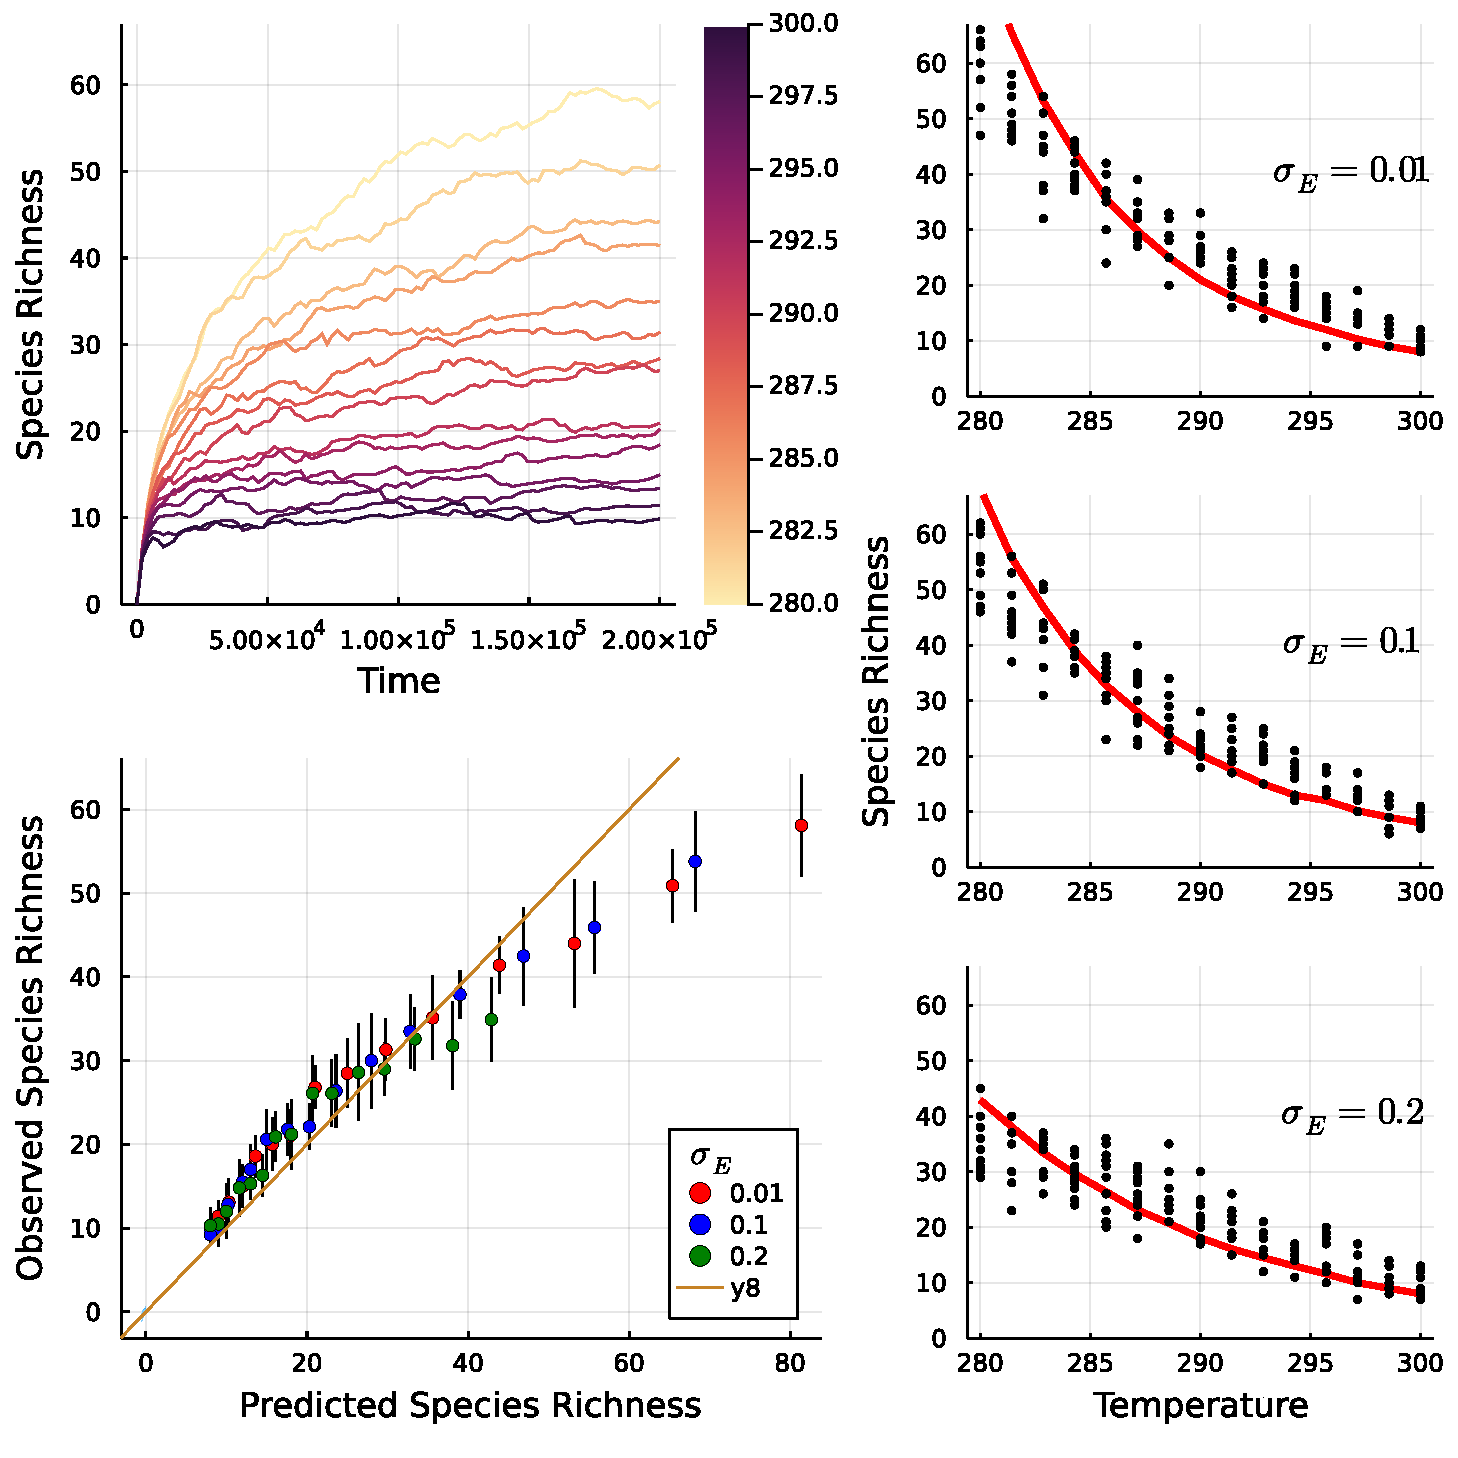
\includegraphics[width = 0.8\textwidth]{docs/Figures/Fig_4.pdf}
    \caption{The assembly of ecosystems at different temperatures is predicted by the analytical feasibility condition. A) Trajectories of species richness over assembly across temperature at a single level of variation in $E$ ($\sigma_a = 0.01$). Each line is the average species richness over time at a given temperature. Species richness is seen to saturate over time, with systems assembling at higher temperatures having lower species richness. B) The observed final species richness reached by the assembly simulations plotted against the analytical predictions of \cref{EQ:P_feas_Temp}. Each point is the average species richness across the 5 replicates with error bars showing the standard deviation. The blue line and shaded region represent the 1:1 line of predictions and observations, representing a probability threshold of \SI{1e-10}, with the shaded region corresponding to the richness predicted by thresholds between \SI{1e-8}-\SI{1e-12}. Overall the predictions and observations of species richness match well, with most of the points variation falling within the predicted bounds, though there is a tendency for the actual species richness to be above and bellow the predictions at low and high species richness respectively. C-E) The species richness - temperature relationship at 3 levels of variation in $E$. Each points represents the species richness reached by a single assembly simulation with the red line and shaded area representing the predicted species richness at a threshold of \SI{1e-10} and within the bounds \SI{1e-8}-\SI{1e-12}. Overall the observed species richness and predictions match well with most observations falling within the prediction bounds. Only at the extremes of temperature (e.g. at 280K in (C)) do the observations significantly fall outside the prediction bounds.}
    \label{Fig:Temperature_assembly}
\end{figure}

\section{Discussion}

We show how variation in thermal sensitvity alters the species-richness relationship
    • We show the two moments of thermal sensitvtiyies have two effects, contoling the direction and the unimodality of thermal response. 
    
This variation is relevant to empirical distriobutons of thermal sensitvties which have enough variation to alter the thermal response of species richness
    • This is expected given previous work showing variation in E
    
Our results are robust to relaxations of the assumptions of our model. 



Our work shows how temperature may affect the feasibility of ecosystems. This is linked to empirical work (cite petchey, new nat-evoeco paper ect.) which has show temperature to be important in  ecosystems. Our work provides a mechanistic understanding of these processes, that temperature, through its action of species demography reduces the ability of species populations to survive. This forms the basis for understanding other dynamic measures and their response to temperature.  

Our work also links this very clearly to the species richness in ecosystems, showing how temperature, though its effect on demographics limits the number of species that can co-exist. This advances our understanding... . Matches the variation in Nsp vs Temp we see 

Our results demonstrate the clear importance of both the average and variance in thermal sensitivity in determining feasibility. Furthermore, this result is remains when we allow systems to assemble with full GLV dynamics suggesting they are fairly robust. This is important given previous work not including variation and work that has shown the simple monotonic TPCs predicted by MTE are not suitable.

Our work highlights the potential of this kind of approach. By considering variation in thermal response traits we can more accurately understand how whole systems respond. This is an important extension of theory of whole ecosystem responses to perturbation which often struggle to realistically portray perturbations. Future work should aim to extend this approach to other measures, especially recent work looking at the sequential collapse of ecosystems. 

Our work has some caveats. As with any study using GLV the applicability of the model is questionable. The simple mass-action dynamics may nor be suitible for systems like microbial cross-feeding networks where more complex dynamics dominate. The key here is for future work to see if the holisitic insights from this model hold up in these situations, for example does the shape of the thermal sensitivity distribution  have the same effect?

In conclusion...

\newpage
\section{Supplementary Material}

\subsection{Mean-field approximation} \label{SI_Sec:Meanfield}

This approximation works by considering interaction term from \cref{EQ:GLV}, which we can rewrite as:

\begin{equation} \label{EQ:mean_int} 
    \sum^N_{i \neq j} a_{ij} x_j = (N-1) \bar{a x} = (N-1) \bar{a} \bar{x} + (N-1) \text{cov}(a,c),
\end{equation}

where the bar notation, $\bar{\cdot}$, represents the average of that quantity over all $N$ species in the system. \Cref{EQ:mean_int} partitions the effects of interactions on the $i$th species into the average effect across the system, $\bar{a} \bar{x}$, and the covariance between heterospecific's biomass and the strength of interactions, $\text{cov}(a,x)$. The mean-field approximation assumes that this second term is negligible, which is equivalent to saying that any individual interaction between the focal species and another species population has little effect on that heterospecific's biomass. We also assume here that the system we consider is large ($N \gg 0$), meaning that the difference between the average biomass across the system and that of heterospecifics is small (as it is in the order $N^{-1}$) and can thus be ignored. For simplicity we make the further assumption that intraspecific interactions are constant across species, setting $a_{ii} = 1$ (though this assumption can be relaxed for the mean-field approximation (REF)). Combining \cref{EQ:GLV,EQ:mean_int} we can then express population dynamics in terms the average interaction strength, giving the full mean-field model:

\begin{equation} \label{EQ:MF}
    \frac{1}{x_i} \frac{dx_i}{dt} \approx r_i - x_i - (N-1)\bar{a}\bar{x}.
\end{equation}

By setting \cref{EQ:MF} equal to $0$ and solving for $x_i$ we then obtain an expression for equilibrium biomass (see \cref{SI_Sec:Meanfield}):


\subsection{Feasibility simulations} \label{SI_Sec:Feas_sims}

\subsection{Derivation of thermal response distributions} \label{SI_Sec:TPC_dist}

\begin{figure}
    \centering
    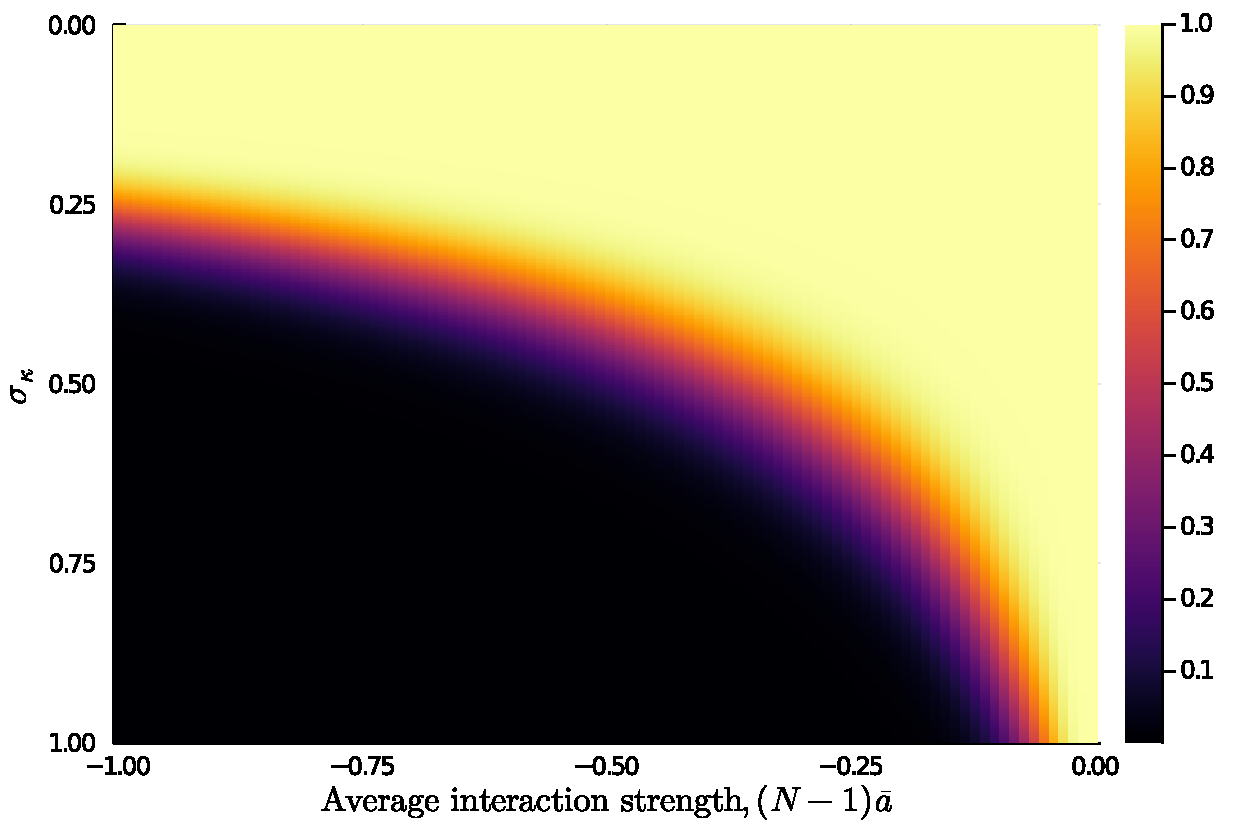
\includegraphics[width = 0.6\textwidth]{docs/Figures/Fig_2.pdf}
    \caption{\textbf{The probability of feasibility $P_{feas}$ as a function of interaction strength and variation in normalised carrying capacity $\sigma_{\kappa}$}. Feasibility shows the same general pattern as \cref{Fig:Feasability_Bound}, decreasing as interactions become more negative and as the variation in $\kappa$ increases (reducing the chance that all species meet the criteria in \cref{EQ:Feas_sp}). $P_{feas}$ is calculated using \cref{EQ:P_feas} setting $N=50$ and allowing $\sigms_{\kappa}$ and $\bar{a}$ to vary such that $\sigma_{\kappa} \in [0 - 1]$ and $\bar{a} \in [-1 - 0]$}
    \label{Fig:P_feas}
\end{figure}

\section{old_intro}
One aspect of temperature that is particularly important is how it affects ecosystem dynamics, the process through which the structure of ecosystems change over time (REF). Ecologists have long been interested in ecosystem dynamics, especially in what they tell us about the ability of ecosystems to persist though time and respond to environmental perturbations (such as temperature)(REF). Though stability, defined as the ability of system to return to some state following a perturbation (REF), has been the focus of much of this research, a whole host of other dynamical measures have also been defined such as reactivity (the strength of the initial response of an ecosystem to a perturbation; REF), resilience (the asymptotic rate of return to equilibrium following a perturbation) and feasibility, which we focus on here. 

An ecosystem is defined to be feasible if there exists a fixed point at which all populations within have positive biomass, that is, all species in the system are able to coexist at equilibrium (REF). Feasibility has recently been highlighted as an important ecosystem property due its role as a prerequisite for other aspects of ecosystem dynamics (e.g. stability, resilience, and reactivity mentioned above). This is because by definition, only the properties of fixed points that actually exist (i.e those guaranteed by the feasibility of a system) are relevant to ecosystem dynamics (REF) or in other words, a system must be feasible in the first place for many of these other dynamic measures to have meaning. Recent work has revealed the importance of species' functional traits (e.g. growth rates and interactions) in determining feasibility, showing how the feasibility condition places a constraint on these trait values within ecosystems. Importantly this work has also linked the feasibility of systems to the number of species they contain (REF) which combined, suggest that we may be able use feasibility as a way to explore patterns of species richness and link them to species traits (REF). 

Though no previous work has looked directly at the relationship between feasibility and temperature, there have been other attempts to understand the thermal responses of whole ecosystem properties such as ecosystem metabolism and local species richness (REF). Broadly this work has tended to use the simplifying assumption of constant temperature dependence, that all populations and traits have the same response to temperature. This allows the derivation of simple analytic predictions which often show a single monotonic (i.e. strictly increasing or decreasing) temperature response (REF). However, this approach has been met with criticism due to both work demonstrating widespread variation in thermal sensitivity of across different demographic processes and taxa and the evidence showing that many of these properties actually demonstrate uni-modal (i.e. peaked) thermal responses. Furthermore a growing body of work shows how important this variation in thermal responses (often referred to as "mismatches") can be in determining the dynamics a number of ecological contexts such as of predator-prey (REF), and virus (REF) and parasite-host (REF)  systems.  

\end{document}
